% PROJECT PROPOSAL TEMPLATE
%
% This document was prepared for use with pdflatex.

% Lines beginning with a % are comments.
\documentclass[a4paper,12pt]{article}

% The amsfonts package contains some useful mathematical symbols
\usepackage{amsfonts}

% The graphicx package allows you to import JPG and PDF images
\usepackage[pdftex]{graphicx}

% The enumerate pachage permits fancy enumerated lists
\usepackage{enumerate}

% Setup the page
\topmargin -1.5cm
\textheight 25.0cm
\oddsidemargin -0.0cm
\textwidth 16.5cm
\pagestyle{plain}
\setcounter{page}{0}
\linespread{1.3}

\begin{document}

%*******************************************************************
% Draw the title page
% The only things you are likely to need to edit are marked with
% a **** comment ****
\begin{titlepage}
\vspace{-1.5cm}
\begin{center}

\includegraphics[width=2cm]{ualogo_colour.jpg}
\vspace{1cm}

\textbf{\large THE UNIVERSITY OF ADELAIDE}\\

\textbf{SCHOOL OF ELECTRICAL \& ELECTRONIC ENGINEERING}

{\small ADELAIDE, SOUTH AUSTRALIA, 5005}

\vspace{1.5cm}
\textsc{Implementation Plan}
\vspace{1cm}

% **** Insert your project title here ****
\textbf{\LARGE Project Title}

\vspace{1cm}
% **** Insert the group members' names here ****
{\Large Group Members}

\vspace{4cm}
\textbf{\large ELEC ENG 4039 A/B HONOURS PROJECT}

\vspace{1ex}
\setlength{\linespread}{1}
\textbf{B.E. in Electrical and Electronic Engineering\\
B.E. in Computer Systems Engineering\\
B.E. in Telecommunications Engineering\\}
\end{center}

\vfill
Each student at Level IV of the course in Electrical and
Electronic Engineering, Computer Systems Engineering and
Telecommunications Engineering is required to complete this course.
The course involves approximately 240 hours of project work over the
whole academic year.  Students are assessed on their performance in
the project, a written proposal, this written report, a technical
paper, and two seminar presentations.

\vspace{1cm}
Date submitted:

\vspace{1ex}
Supervisor:

\vspace{1ex}
Signature of Supervisor:
\end{titlepage}
% End of the title page
%*******************************************************************

\newpage
% The \section* command creates a section without a number
\section*{Objectives}
Concisely state the objectives of the project. You should be able to
do this in just a few sentences.

\newpage
\tableofcontents

\newpage
% The \section command creates a numbered section
% Note that there are also \subsection and \subsubsection commands.
\section{Background and Significance}

The first aim of this project is to co-operate with the VLSI class
from Harvey-Mudd College, California, to design and build a MIPS-based
microprocessor.

Microprocessors are electronic devices that contain all the functions
of a CPU on a single integrated circuit. This microprocessor will be
split into a control unit, a coprocessor and a data path. The datapath
contains a fetch, decode, execute and memory stage. The Adelaide team
is designing the 512kB cache for the memory stage. A cache stores
recently used memory data on chip to save slow memory accesses. The
cache is direct mapped, meaning that each datum from memory has a
unique place it can be stored in the cache.

The chip will use a MIPS R2000 instruction set architecture
(ISA). MIPS stands for Microprocessor without Interlocked Pipeline
Stages. The MIPS ISA is a popular RISC microprocessor
architecture. R2000 has 32-bit instructions including various loads,
stores, arithmetic, jumps and branches, shifts, moves and exceptions.

In the production of a microprocessor testing is required on both the
design and the finished hardware.

\section{Project Specifications}

\subsection{Final Deliverables}
\begin{enumerate}[{[D}1{]}]
\item Hardware Presentation of the MIPS-based microprocessor
\item Package of testing tools and report on test results
\item Extension: Report examining low power design alternatives
\end{enumerate}

\subsection{Requirements}
\begin{enumerate}[{[R}1{]}]
\item Hardware demonstration
  \begin{itemize}
  \item Running an interactive program (possibly a Web-server or
    ELIZA).
  \item Robust packaging so that the demonstration is easy to
    move and set up.  
  \item Uses MIPS-based microprocessor.
  \end{itemize}

\item Testing tools
  \begin{itemize}
    \item Software tests of design using either fast SPICE or IRSIM,
      depending on availability.
    \item Documentation for software testing.
    \item Detailed methods of hardware testing.
  \end{itemize}
\item Extension: Report on low power
  \begin{itemize}
  \item Examination of MIPS based microprocessor.
  \item Development of alternative designs to achieve low power.
  \item Examination and evaluation of alternative designs
  \end{itemize}
\end{enumerate}

\subsection{Reporting Requirements}

First Semester
\begin{description}
\item[Week 4 Project Implementation Plan:] A plan detailing what is to
  be accomplished during the project, and how the group intends to do
  it.
\item[Week 5 Proposal Seminar:] Presents and explains the intended
  project including requirements and what will be produced.
\item[Week 8 Critical Design Review:] Evaluate and assess intended
  design(s) for project.
\item[Week 10 Submit Peer Review:] Review another group's project.
\item[Week 12 Project Log Book:] A record of all meetings and time
  spent on the project.
\end{description}

Second Semester
\begin{description}
\item[Week 9 Final Project Report and Technical Paper due:] The final
report covering the completed project and the process of producing it.
\item[Week 10 Final Project Seminars:] A seminar on the completed
project.  
\item[Week 11 Project Exhibition:] Displaying the project to the
public.
\end{description}

%\subsection{Acceptance Criteria}
%
%State how the customer will measure whether the project has been a
%success.

\section{Proposed Approach}

\subsection{System Architecture}

The cache is the focal point of our project. A thorough description of
the memory system being implemented for this project can be found in
\cite{various07}. The MIPS microprocessor was initially designed
by defining an interface and then describing all modules in verilog
using a development tool called ModelSim. Once the verilog system was
completed and verified work began on translating the verilog code into
schematics. The schematics are currently in the process of being
developed and using a VLSI design application called Electric8.04. The
design process will be elaborated in Section 3.2.

Given in Figure~\ref{cacheblock} is the current block diagram of
the cache system. The cache is comprised of:
\begin{enumerate}
\item Cache Controller
\item Cache RAM
\item Data Out
\item Byte Enable
\item Various simple logic components including multiplexers,
  inverters, and OR gates.
\end{enumerate}

\begin{figure}
\centering 
%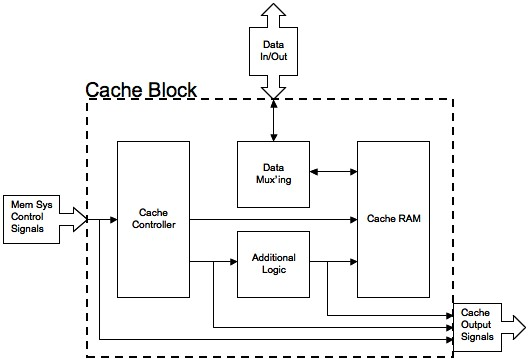
\includegraphics[width=\textwidth]{cacheblock}
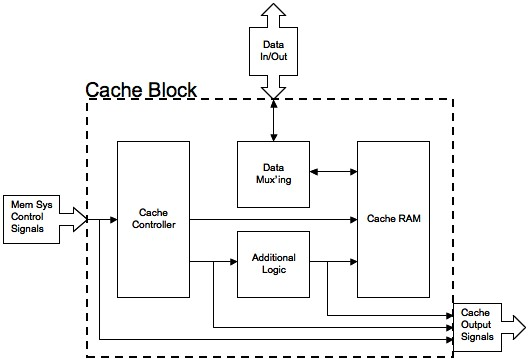
\includegraphics[width=\textwidth]{cacheblock}
\caption{Block diagram of the MIPS cache.}
\label{cacheblock}
\end{figure}

The Adelaide team will be involved in the continued design and
verification of the Cache Controller and the Cache Ram. These modules
are described in further detail in Figure~\ref{cachcontroller} and
Figure~\ref{cacheram} respectively.

\subsection{Cache Controller}

This module comprises the following components: 
\begin{enumerate}
\item Address Tag Data Logic
\item Controller State Logic
\item Inverters, OR gates and flops
\end{enumerate}

\subsection{Cache Ram}

This module contains the following components:
\begin{enumerate}
\item 64-bit Decoder
\item Cache Signal Buffers
\item SRAM Array
\item Bit Line Conditioning
\item Write Driver
\end{enumerate}

\begin{figure}
\centering 
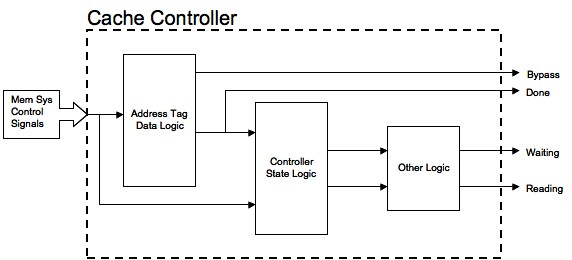
\includegraphics[width=\textwidth]{cachecontroller}
\caption{The MIPS cache controller module.}
\label{cachecontroller}
\end{figure}

\begin{figure}
\centering 
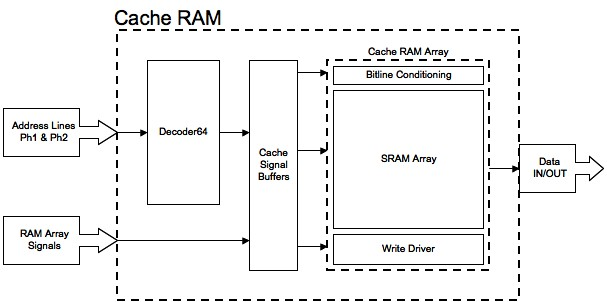
\includegraphics[width=\textwidth]{cacheram}
\caption{The MIPS cache ram module.}
\label{cacheram}
\end{figure}

\subsection{Design Processes}

Figure~\ref{designprocess} describes the methodology that will be
followed to complete the stages of development of the cache
system. The first stage involves starting with the verilog
specification that has already been developed and verified. This
starting point involves learning the verilog hardware description
language and then determining what modules were used and the overall
interface for the memory system. The verilog code was developed using
ModelSim and so familiarity with this development environment is a
requirement.

The next stage of the design flow involves designing schematics from
the verilog code. This will be achieved by using the VLSI design suite
Electric. Once the schematics are designed a verilog deck, containing
the schematic netlist of a module will be extracted and inserted in
place of the original verilog description for that module. This will
enable checking that each schematic that has been designed integrates
with the interface and is logically correct.

Once the schematics have been verified, layouts of the schematics will
commence. A similar testing procedure will be conducted to the
schematics for the layouts in addition to the MOSIS rules, Schematic
vs Layout verification features built-in to Electric.

At present, the intended further testing procedure involves generating
IRSIM command files and spice test files from the verilog
code. Verilog is only designed to conduct logical testing of
circuitry.This is, therefore, an important stage to complete since
IRSIM will be allow evaluation of delays and critical paths within the
circuitry. `Fast Spice' will also be used to check on behaviour of
circuitry that is significant to analogue design.

\begin{figure}
\centering 
\includegraphics[width=\textwidth]{designprocess}
\caption{Flow chart of the design process for the project.}
\label{designprocess}
\end{figure}

%MELS SECTION

\section{Project Plan}

\subsection{Interim Deliverables}
\begin{enumerate}[{[ID}1{]}]
\item Cache designs for MIPS-based microprocessor
\item MIPS microprocessor in package
\item Software for MIPS
\item Documentation: 
  \begin{itemize}
  \item Chip report (HMC requirements)
  \item Reporting requirements
  \end{itemize}
\end{enumerate}


%\subsection{Milestones}
% The \label command marks a section (or a table, equation or figure) so 
% that it can be referenced elsewhere in the text.
%\label{sec:milestones}
%\begin{description}
%\item[M1 01/01/07:] list the key milestones for your project.
%\item[M2 01/01/07:] each final deliverable will have a deadline. These
%  should be milestones.
%\item[M3 01/01/07:] assign deadlines to the most important interim
%  deliverables. These should also be milestones.
%\end{description}

\subsection{Work Breakdown}

This section is to be read in association with the accompanying Gantt Chart.

\begin{enumerate}
\item \textbf{Project Planning:} (26th Feb 2007 - 2nd March 2007) 

\item \textbf{Devise Test Plan:} (3rd March 2007 - 5th March 2007)

\item \textbf{Block Schematic Simulate:} (milestone: 5th March 2007)

\item \textbf{Project Implementation Plan:} (milestone: 22nd March 2007)

\item \textbf{Block Level Design Validation:} (6th March 2007 - 25th March 2007)

\item \textbf{Proposal Seminar:} (milestone: 26th March 2007)

\item \textbf{System Level Design Validation:} (27th March 2007 � 29th April 2007) 
  \begin{enumerate}[a)]
    \item EDA tools (Rob)
    \item VCD parse (Joel)
    \item Verilog trace writes (Mel) 
    \item Snoopgen (Rys)
    \item Testing (All)
  \end{enumerate}

Tasks a) to d) can be done in parallel to each other by assigned group members. Testing will commence after the implementation of each task.

\item \textbf{Critical Design Review:} (milestone: 30th April 2007)

\item \textbf{Project Extension Planning:} (1st May 2007 � 10th May 2007)

\item \textbf{Extensions:} (18th May 2007 � 13th August 2007)
The project extension can be divided into 4 different parts:
  \begin{enumerate}[a)]
    \item Low Power Design (Rob and Rys)
    \item Interactive Demonstration Program for the chip (Joel)
    \item Peripherals for the chip (Rys) 
    \item Packaging design (Mel)
  \end{enumerate}

Research and implementation of the four different parts will commence in mid of May. Each part of the extension will be implemented by the assigned group member. These extensions can be done in parallel to each other. The testing of each part will begin after the completion of design and implementation.

\item \textbf{FPGA Testing:} (2nd  September 2007 � 15th September 2007)

\item \textbf{System Integration and Testing:} (15th September 2007 -  21st October 2007)

\item \textbf{Final Individual Report:} (milestone: 4th October 2007)

\item \textbf{Final Seminar:} (milestone: week 10 and 11)

\item \textbf{Project Exhibition:} (week 12)
\end{enumerate}

\subsection{Activity Schedule}
%%TODO PUT IN RIGHT SPOT 
\begin{figure}
\centering
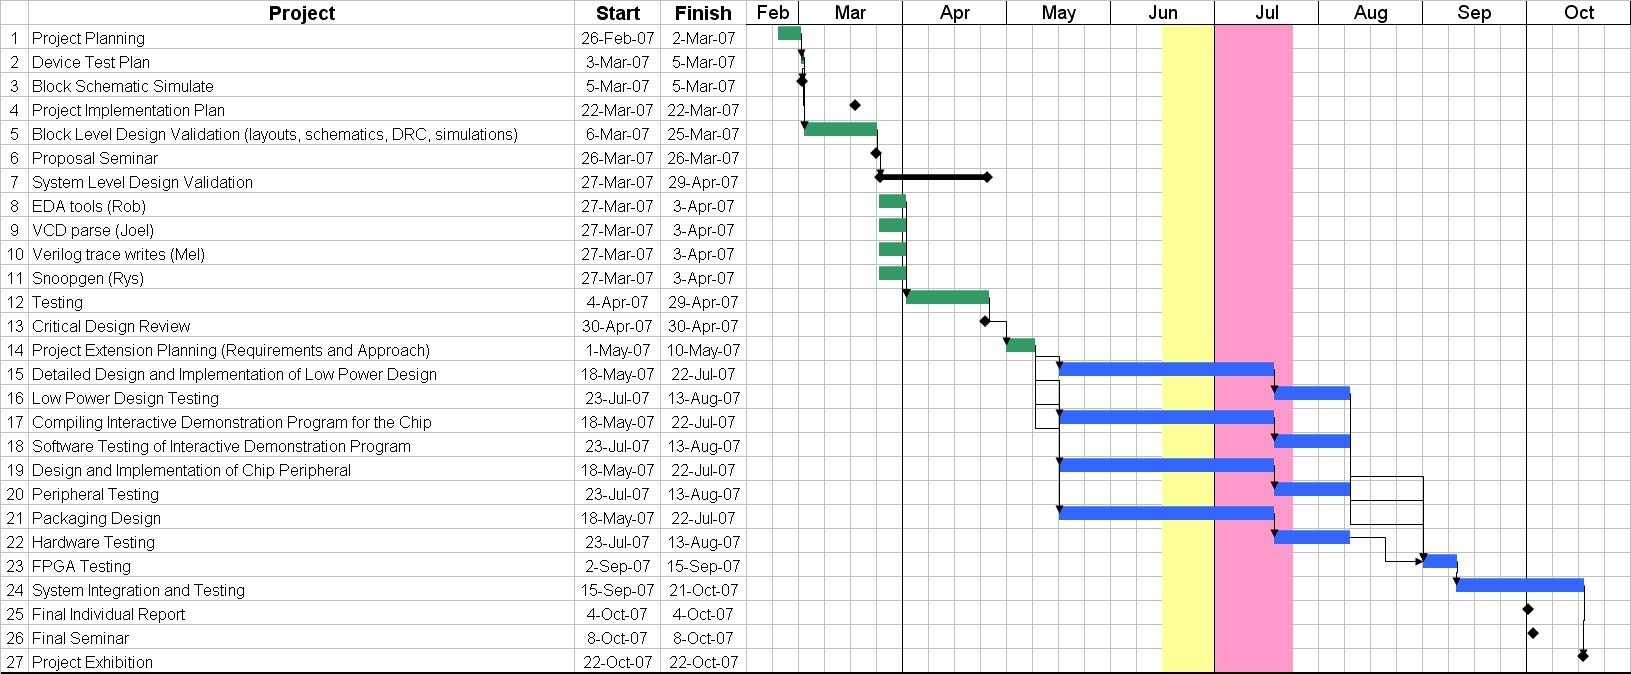
\includegraphics[width=\textwidth]{gantt-chart}
\caption{Schedule}
\label{gantt-chart}
\end{figure}


\section{Risk Analysis}

The potential risks in this project are shown in Table~\ref{risks} and some planned approaches are described in this section.

\begin{table}[h]
\begin{tabular}{|l|l|l|l|}
  \hline
  % after \\: \hline or \cline{col1-col2} \cline{col3-col4} ...
  \textbf{Risk} & \textbf{Chance} & \textbf{Impact} & \textbf{Rating} \\
  \hline
  \hline
  1. Project falls behind schedule & moderate & moderate & moderate\\
  \hline
  2. Communication failure & low & high & moderate\\
  \hline
  3. Design bugs & moderate & moderate & moderate\\
  \hline
  4. Faulty hardware parts & low & moderate & low\\
  \hline
  5. Unavailability of resources & moderate & low & low\\
  \hline
  6. Absence of team members & low & low &low\\
  \hline
  7. Change of supervisor & high & low & moderate\\
  \hline
  8. Changing requirements & moderate & low & low\\
  \hline
  9. Fabrication grant is not awarded & low & high & moderate\\
  \hline
\end{tabular}
\caption{Summary of potential risks.}
  \label{risks}
\end{table}

\begin{enumerate}
\item \textbf{Project falls behind schedule:} Some of the project milestones are set by the Harvey Mudd College team. Thisproject will be very heavily loaded in the first semester. It also requires knowledge of microelectronics circuit design, circuit verification, computer architecture etc., therefore the team needs some extra reading and practice on tools that we are using, prior to the commence of the actual work for achieving the target project milestones. Even though this project was commenced before the beginning of the semester, the team member will be required to spend extra time and effort in order to meet the deadlines. Considering the project extensions in the second semester, the low power extensions are lower priority, Rys and Rob can be reallocated if project severely falls behind schedule.

\item \textbf{Communication failure:} This project is conducted in collaboration with the Harvey Mudd College team in California. Regular contact with the other teams in California is important. Design reviews also will be conducted with the aid of video conferencing. Therefore, alternative contact information other than university email, such as telephones and faxes are necessary to prevent unexpected communication failure. Besides, weekly project meetings in Adelaide will include status review, each member can specify their progress and plan in order to prevent digression and allows clarification on actions open to misinterpretation.

\item \textbf{Design bugs:} The cache circuit design was brokedown into blocks and each member are allocated to different blocks to test their functionalities. In order to ensure the reliability of the overall chip design, designing high coverage test benches are required for design bugs detection. Careful simulation checks are very crucial, if test bench flags error, the design will be reviewed to resolve the problem. All blocks should be tested prior to the final testing of the integrated cache circuit. Besides, the Adelaide team will attempt extra system-level verification. Both Adelaide and US teams are performing independent system level tests to enhanced system reliability.

\item \textbf{Faulty hardware parts:} The team is expecting the real chip to be delivered in the second semester to proceed with the project extension on low power design and hardware demonstration. Any faulty hardware part will affect the testing results of the chip. By foreseeing the risk, the FPGA is another alternative if hardware fails. Our backup plan is to use FPGA to demonstrate our project in the end of the year if chip fails to perform as what we expected. 

\item \textbf{Unavailability of resources:} Some software tools may become unavailable in the computer in CATS and EM211. We should submit support requests as soon as problems are noticed. Meanwhile, the team will work on other tasks until the tools become available to reduce the impact. It may be possible to use other tools, e.g. The school of Engineering has multiple Verilog simulators.

\item \textbf{Absence of team members:} If a team member is sick or burdened with other commitments, other team members must continue productive work. The project schedule will be reassessed if necessary, less priority extension might be omitted from project plan.

\item \textbf{Change of supervisor:} The current supervisor, Dr. Branden Phillips will be away in the second semester and his supervising job on this project will be taken over by Dr. Brain W. Ng. It is the responsibility of the team to update the supervisor on the progress of the project, and also be prepared for any adjustment in running project.

\item \textbf{Changing requirements:}The cache circuit will be incorporated into the MIPS microprocessor which is still currently being developed. The team is expecting the change of requirements for the cache circuit throughout the circuit design process in order to optimize the overall chip performance.

\item \textbf{Fabrication grant is not awarded:} There is a possibility that the MIPS microprocessor will not be granted for fabrication in April or later. This will result in a great impact on out project plan for the second semester as we are expecting to get the real chip for testing and further improvement on low power design. Besides, the project demonstration in week 12 required final product to be presented. As a backup plan, we use FPGA for prototyping the MIPS microprocessor design so that it can perform whatever logical function is needed. A FPGA board will be purchased towards the beginning of semester one.
\end{enumerate}



%END MELS SECTION

\section{Budget}

There is an allocation of $250 per student, making the team budget
$1000. At this stage we have identified only one item to purchase,
that being a Xilinx XCV2P Virtex-II Pro FPGA board. The cost is
US\$299, approximately \$370. 

\begin{table}[h]
\begin{tabular}{|l|c|c|c|c|}
  \hline
  \textbf{Item} & \textbf{Cost} \\
  \hline
  \hline
  Budget allocation & \$1000 \\
  \hline
  Xilinx FPGA & -\$500 \\
  \hline
  \hline
  \textbf{TOTAL} & \$500 \\
  \hline
\end{tabular}
\caption{Project budget. }
 \label{budget}
\end{table}

% The 99 parameter tells LaTeX there are at most 99 references.
\begin{thebibliography}{99}

% Use this format of references to online material
\bibitem{Green07} C.~A.~Green, \emph{Final Year Honours and Design
  Project Handbook}, 2007, http://www.eleceng.adelaide.edu.au/students/undergrad/courses/4039/material/notes/

\bibitem{various07} Various, \emph{HMC-MIPS Wiki Design Sketches},
2007, http://code.google.com/p/hmc-mips/wiki/DesignSketches

\end{thebibliography}

%\newpage
%\section*{Glossary and Symbols}
%
%\begin{description}
%\item[Discursive Viscosity:] The average number of jargon terms per
%paragraph.
%\item[RNS:] Residue Number System
%\item[TLA:] Three Letter Acronym
%\item[\(\psi\):] Discursive viscosity
%
%\end{description}

\end{document}
